\chapter{Evaluation}

This chapter will discuss the evalution and testing of the system and its components. The next sections will cover the evaluation of the frontend, backend and the LLM used. This chapter will then conclude with a discussion on the client feedback received at the end of the project.

\section{Frontend Testing}

Frontend testing was mainly conducted through manual testing, done at the same time as the development of said components. While initially the plan was to use automated testing, the time constraints, complexity of components and lack of experience with any testing frameworks led to the decision to use manual testing instead. 

To ensure some level of robustness in the testing procedure, a checklist or a list of test cases was created for every created component. After finishing development, this list would then be used to ensure the component wasa working as intended. To have a more structured approach, the test cases were usually written using the Gherkin syntax, which follows the Given-When-Then format, allowing for better definition of the test cases \parencite{gherkin}. 

An example of some test cases for the selection of records to be shared in a share link is shown below:

\begin{lstlisting}[language=Gherkin, caption=Test cases for selecting records to be shared in a share link]
    Feature: Record selection for share link

    Scenario: User selects all record types to be shared
        Given the user is on the share link page
        When the user selects the top checkbox to select all record types
        Then all record types should be selected for sharing
        And the all children checkboxes should be selected as well 
    
    Scenario: User selects specific record types to be shared
        Given the user is on the share link page
        When the user selects a specific record type to be shared
        Then only the selected record types should be selected for sharing
        And the respective children checkboxes should all be selected as well

    Scenario: User selects specific children records to be shared
        Given the user is on the share link page
        When the user selects specific children records to be shared
        Then only the selected children records should be selected for sharing
        And the respective parent checkbox should not be selected
        And the top child checkbox should not be selected
\end{lstlisting}

And the respective frontend result of these test cases can be seen in figures~\ref{fig:test1},~\ref{fig:test2} and~\ref{fig:test3}. The first figure shows the selection of all record types, the second figure shows the selection of specific record types and the third figure shows the selection of specific children records.

\begin{figure}[htbp]
    \centering
    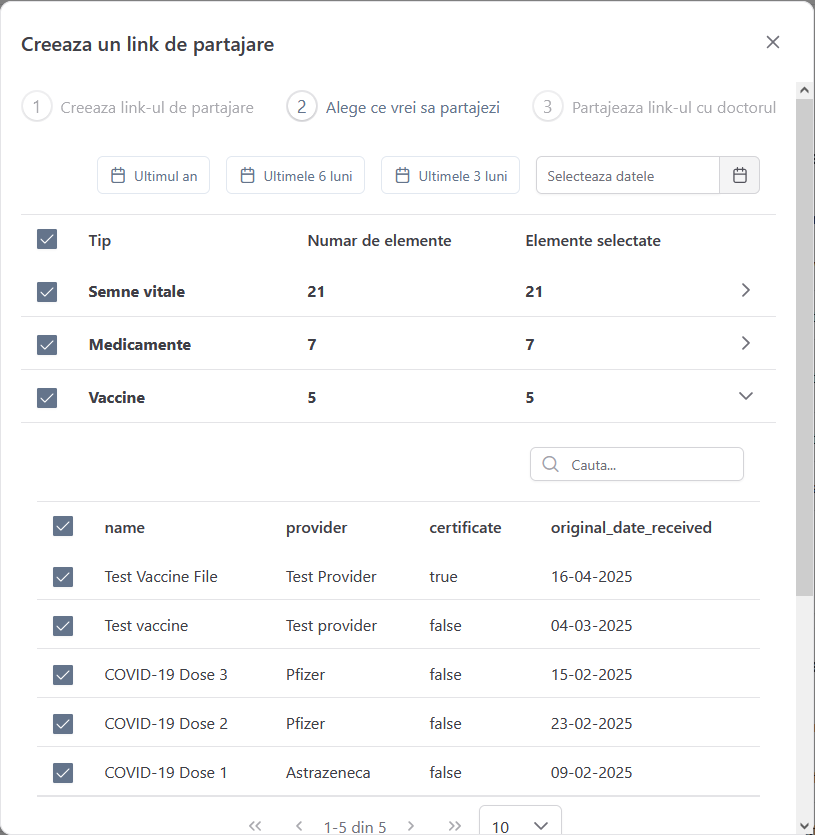
\includegraphics[width=\textwidth]{TestCase_All.png}
    \caption{Test Scenario \#1}\label{fig:test1}
\end{figure}


\begin{figure}[htbp]
    \centering
    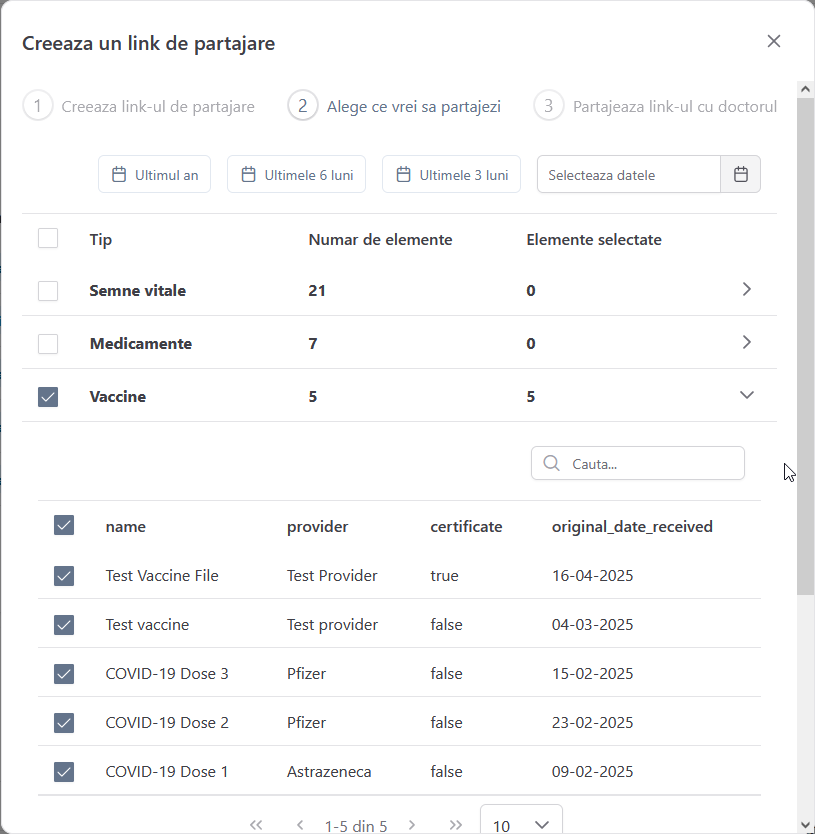
\includegraphics[width=\textwidth]{TestCase_One.png}
    \caption{Test Scenario \#2}\label{fig:test2}
\end{figure}

\begin{figure}[htbp]
    \centering
    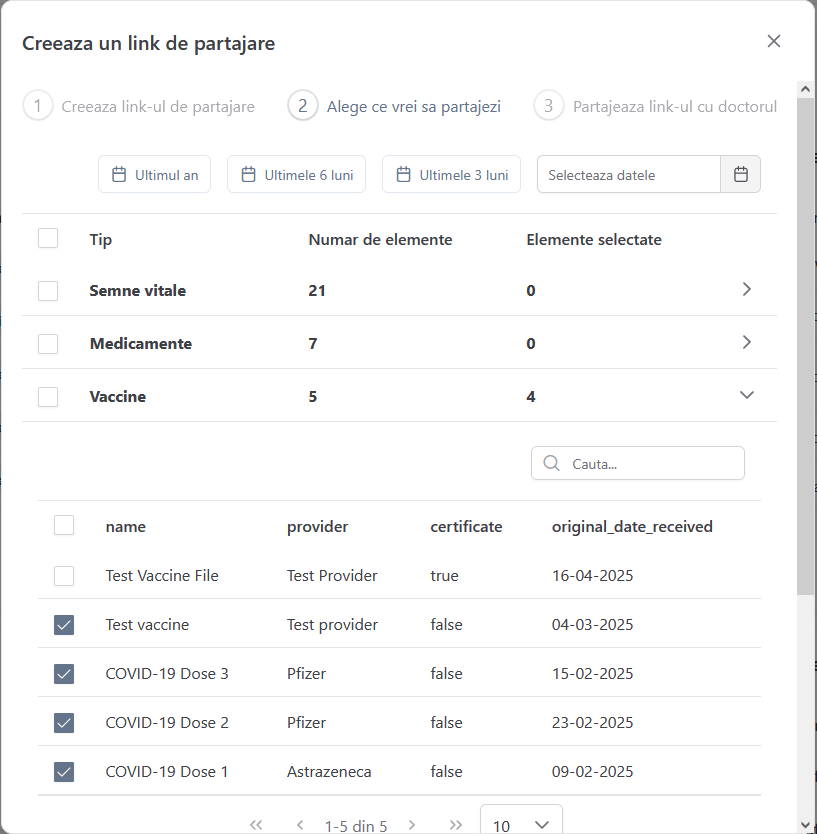
\includegraphics[width=\textwidth]{TestCase_SomeChild.png}
    \caption{Test Scenario \#3}\label{fig:test3}
\end{figure}

\FloatBarrier{}

In addition to the test cases, a site map was created to track all the pages and their respective components, with relationships showing how each page and component is related to each other. This was done to ensure that all components were created and tested properly. In the end, it allowed for a better, high-level overview of the system and its parts, but also for tracking of the overall progress of the project. The site map can be seen in figure~\ref{fig:sitemap}.

\begin{figure}[htbp]
    \centering
    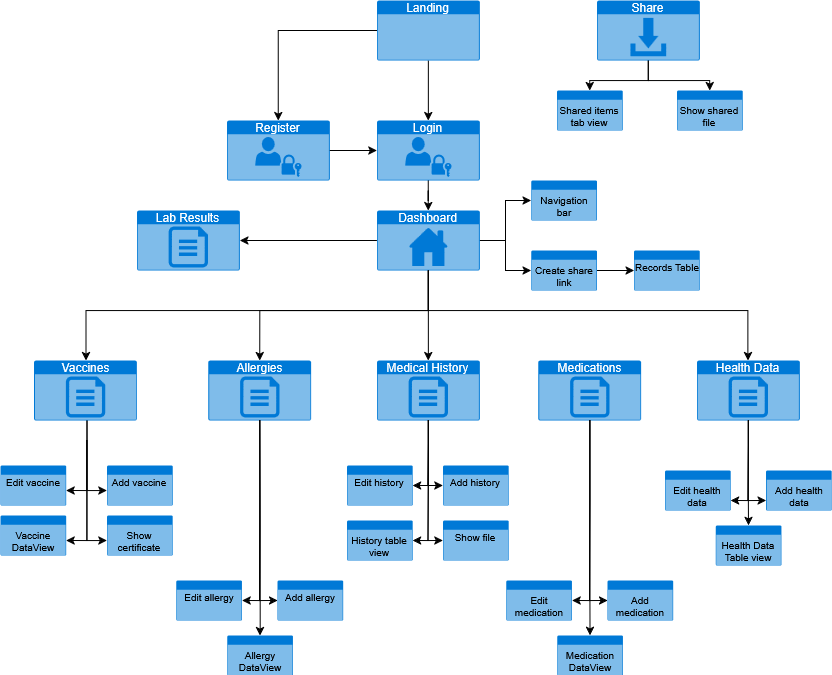
\includegraphics[width=\textwidth]{SiteMap.png}
    \caption{PHR System Site Map}\label{fig:sitemap}
\end{figure}

\FloatBarrier{}

\section{Backend Testing}

\section{LLM Evaluation}
% Research LLM evaluation methods
% Talk about LLM evaluation for Gemini 2.0 Flash

\section{Client feedback}